\chapter{Reflexión de Fuerzas en el dispositivo maestro}
\begin{flushright}
\begin{minipage}{0,7\textwidth}

En este capitulo se presenta el diseño de una tarjeta de acondicionamiento de señal para convertir la corriente sinusoidal que fluye por los motores en una tensión de corriente continua para ser leído con mayor facilidad por el controlador de tiempo real. Posteriormente se presentan resultados experimentales realizados para estimar la relación entre la corriente consumida por los motores y la fuerza producida.

\end{minipage}
\end{flushright}



\newpage
En las últimas tres décadas la investigación en el control de fuerzas ha avanzado significativamente debido al gran interés de dotar a los sistemas robóticos de información y capacidades sensoriales. Los sensores de tacto, fuerza, distancia junto con la realimentación visual permiten la operación autónoma en entornos no estructurados.\\


Desde de las primeras investigaciones en el área de teleoperación el uso de la realimentación de fuerza fue concebido para ayudar al operador humano a manipular objetos en un entorno remoto con un manipulador esclavo. Recientemente se vienen utilizando sistemas robóticos cooperativos consistentes en dos o más manipuladores apoyándose entre s\'i para la realizaci\'on de las tareas.\\

El control de fuerza juega un papel muy importante en el comportamiento y versatilidad de los sistemas robóticos en entornos abiertos dotándoles de una respuesta inteligente en situaciones donde no hay visibilidad y permitiendo la interacción hombre-robot.\\



El control de la interacciones físicas entre el robot y su entorno es crucial para la ejecución de tareas donde el efector final del robot tiene que manipular objetos o realizar tareas en una superficie. Un ejemplo claro puede ser el pulido de una pieza recién pintada de un coche, donde la herramienta de pulido tiene siempre que estar en dirección normal a la superficie de trabajo. Otras aplicaciones donde se requiere el control de fuerza son operaciones de ensamblaje o mecanizado. Una clasificación completa de las tareas que requieren de un control de fuerza, incluyendo aplicaciones no industriales, es prácticamente imposible, debido a la gran cantidad de estas existentes, además de que no sería necesaria dicha clasificación para desarrollar una estrategia para controlar la interacción con el ambiente.\\


\section{Diseño de una tarjeta para medir la corriente en los motores del maestro }

La principal aportación de este trabajo fue la reflexión de fuerzas en el sistema maestro. Como se mencion\'o en el apartado de descripción de la plataforma de teleoperación, el sistema maestro es actuado por motores bifásicos de corriente alterna en cada uno de sus grados de libertad. Las señales de corriente alterna son generadas a través de una de las tarjetas de adquisición de datos del controlador de tiempo real (PXI) y posteriormente amplificadas en una etapa de potencia para suministrar la corriente necesaria a los motores.\\


Dado que el dispositivo maestro está equipado con motores bifásicos de CA que giran en un sentido o en otro dependiendo del desfase de las señales de entrada, el par ser\'a proporcional a la amplitud de la corriente.\\

\begin{figure}[ht!]
\centering
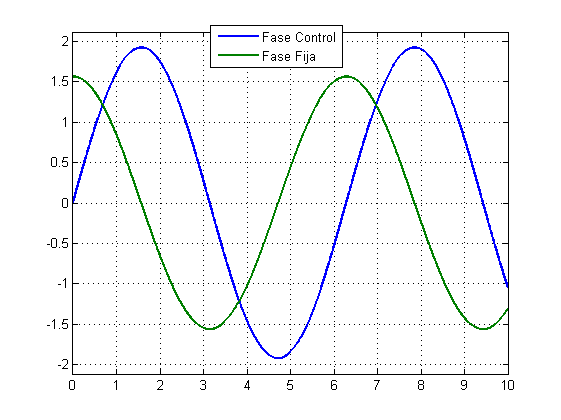
\includegraphics[scale=0.5]{FiguresP/entradaMotores}
\caption{Señales de entrada al motor}
\label{senalesmotor}
\end{figure}


El controlador del sistema esclavo toma mediciones de la fuerza aplicada en cada una de las articulaciones por medio de unos transductores de presión instalados en el interior de los actuadores hidráulicos. La información de los sensores de   presión se encuentra disponible en variables compartidas a través de Ethernet por medio del protocolo UDP.\\



Para reflejar y tener control sobre las fuerzas ejercidas en el dispositivo maestro la idea inicial fue medir la corriente directamente en cada una de las dos fases de cada motor. Un primer intento fue medir directamente el voltaje a través de los sensores de corriente (Sensores CS2.A03 ver figura \ref{fig:sensoresCorriente}) que entregan a su salida un voltaje proporcional a la corriente que circula por cada una de las dos fases. Para obtener una realimentación de la fuerza en cada uno de los cinco grados de libertad disponibles en el dispositivo fueron necesarios diez sensores de los antes mencionados.\\

\begin{figure}[!htb]
\centering
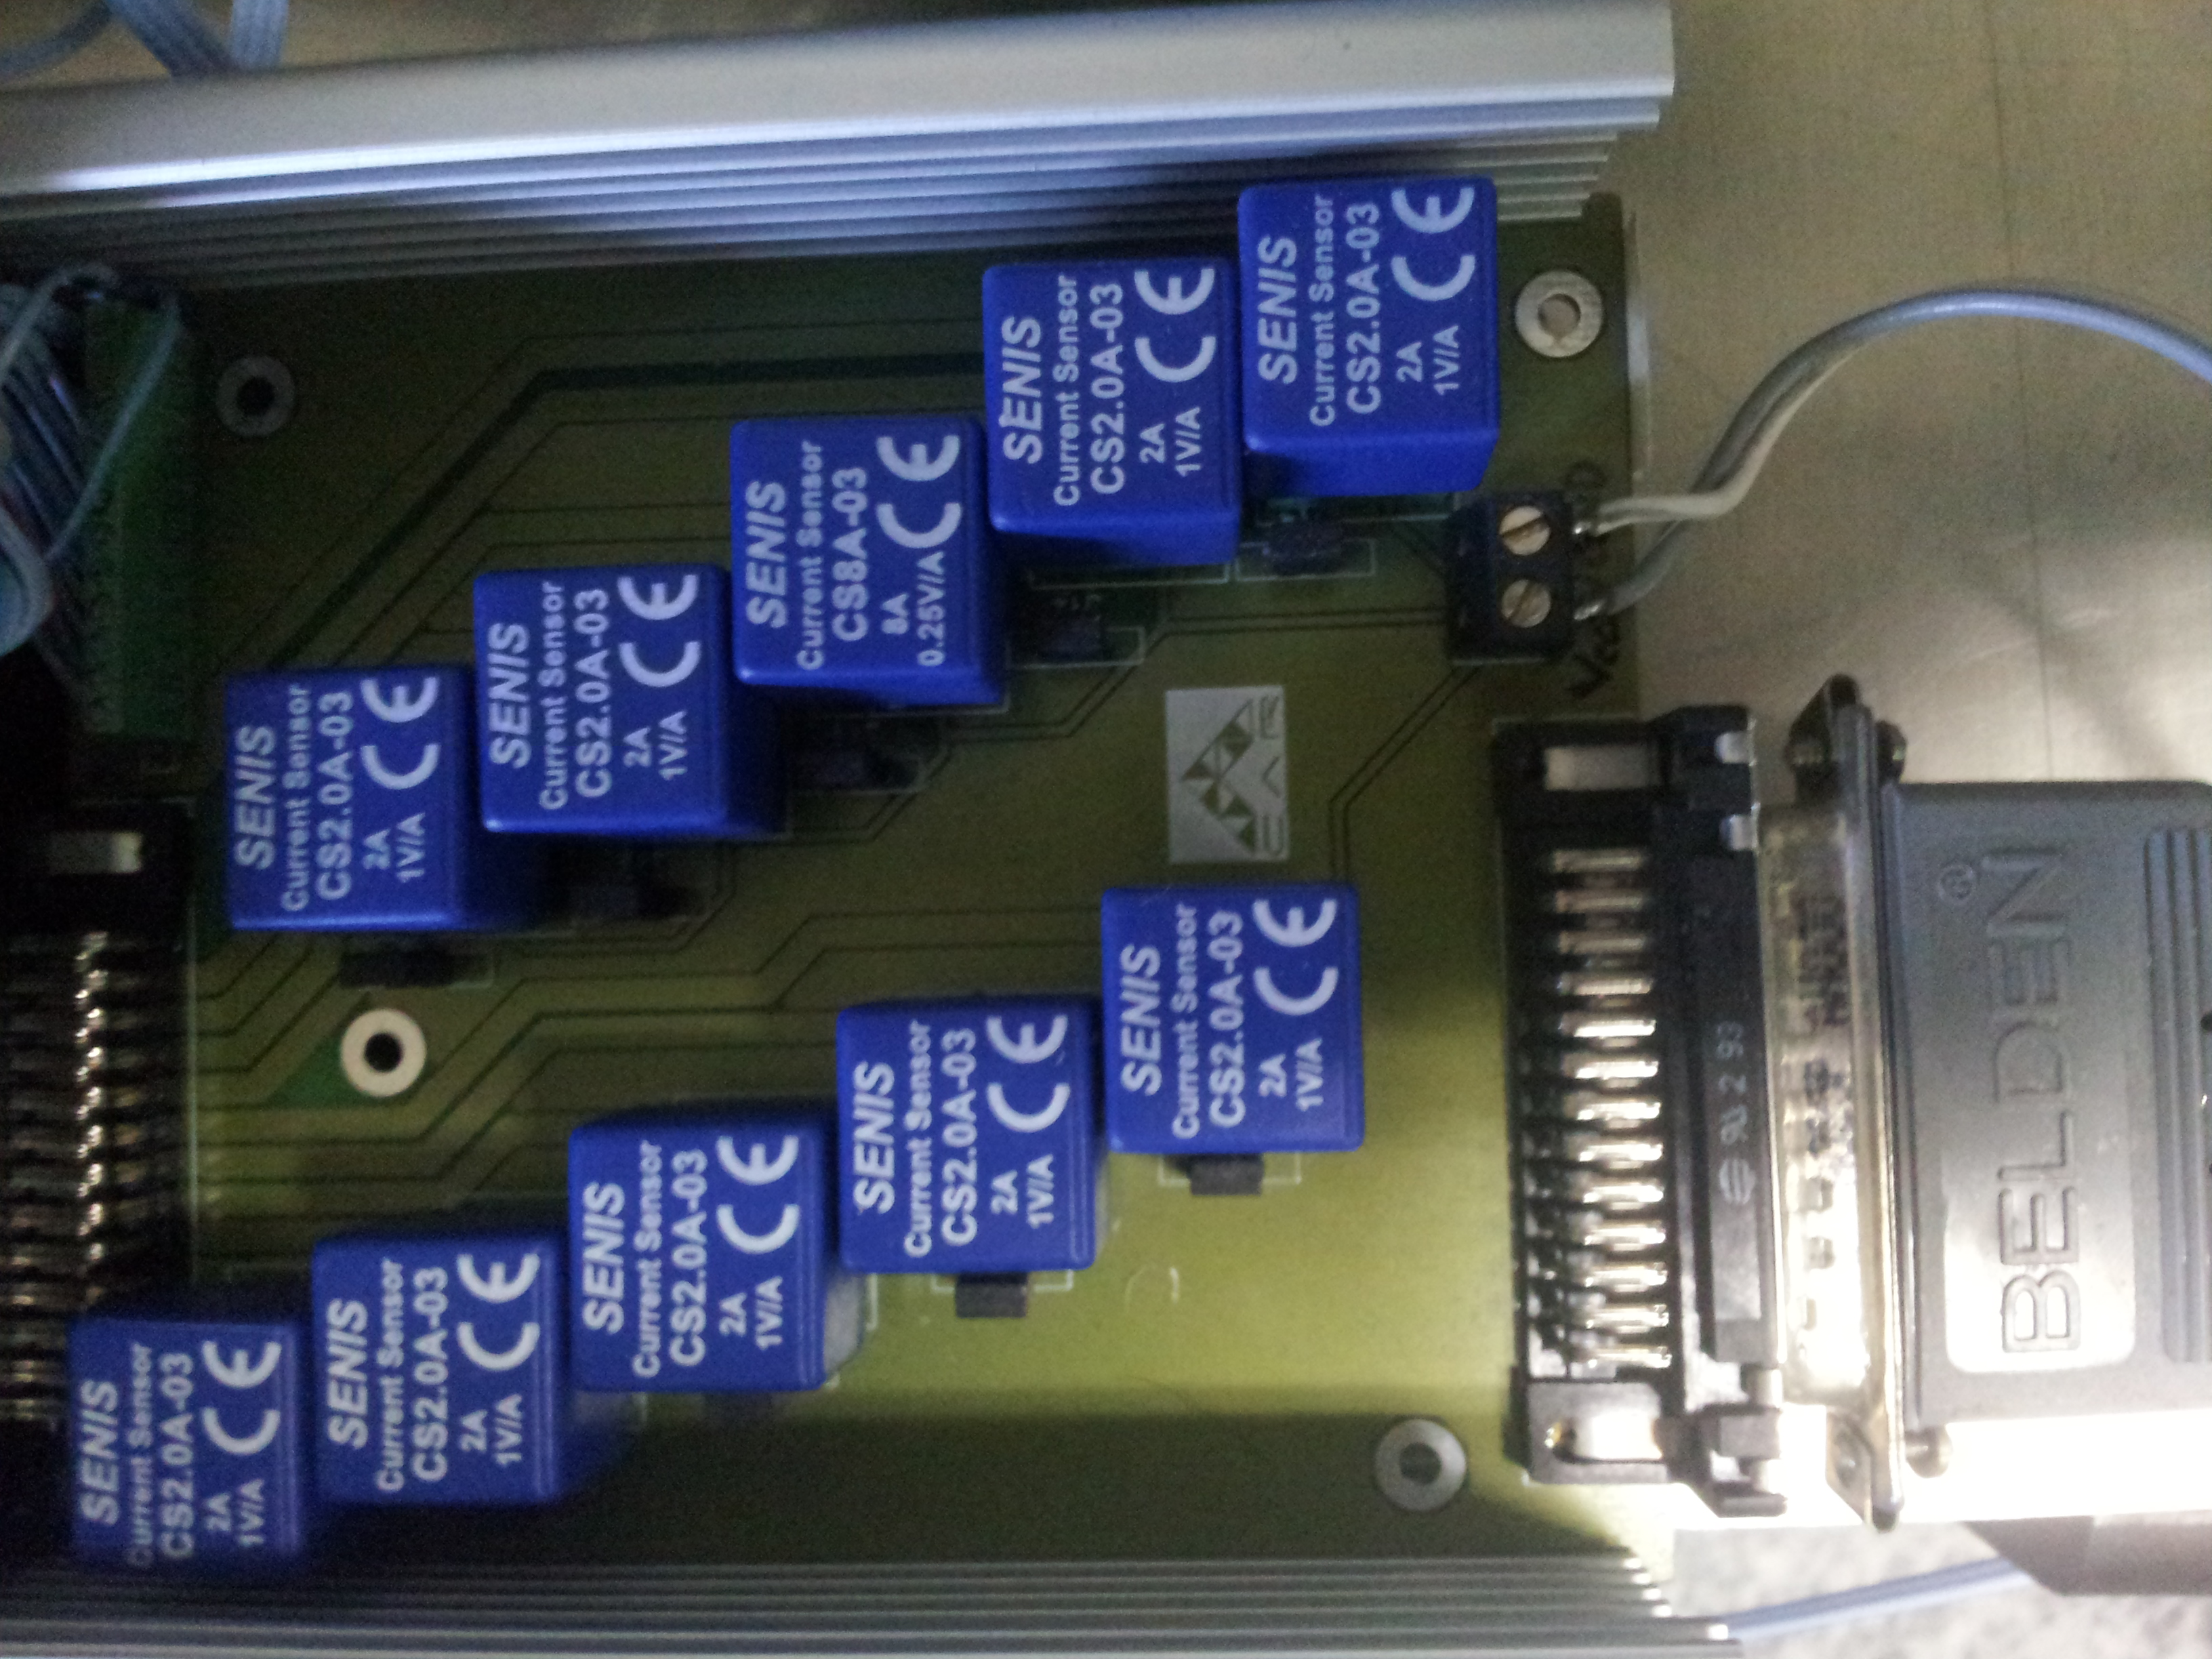
\includegraphics[scale=0.07]{FiguresP/CurrentSensors}
\caption{Tarjeta para leer la corriente a través de los motores del dispositivo maestro}
\label{fig:sensoresCorriente}
\end{figure}


El inconveniente de la propuesta inicial fue que había que tomar las lecturas de tensión en cada uno de los diez sensores. Después medir el desfase entre cada una con lo que ser\'ia necesario agregarle otro módulo de adquisición de entradas analógicas al controlador en tiempo real. Por otra parte había procesamiento excesivo por parte del controlador  para calcular el desfase de las señales de entrada y el valor eficaz vi\'endose afectadas partes críticas dedicadas a la comunicación y al control maestro-esclavo.\\


La solución propuesta fue diseñar un circuito de acondicionamiento capaz de convertir las diez señales sinusoidales provenientes de los sensores de corriente en cinco señales proporcionales al valor eficaz de la onda sinusoidal y con el signo dependiente del desfase de las señales de cada motor. \\

En el circuito de la figura \ref{fig:TarjetaCorriente} se puede observar la propuesta para el acondicionamiento de las señales de los sensores de corriente en los motores, el funcionamiento se describe a continuación:

\begin{description}
\item Un circuito integrado se encarga de calcular el valor eficaz de una de las formas de onda de los sensores de corriente, a la salida del circuito se entrega un valor de corriente directa proporcional al valor eficaz.

\item Por otro parte dos comparadores se encargan de detectar el cruce por cero de ambas señales sinusoidales, entregando un valor digital en cada cruce por cero

\item La salida de los detectores de cruce por cero es conectada a las entradas D y clk de un Flip-Flop tipo D con la finalidad de detectar el desfase de las señales, en caso de la fase de control este en adelanto con respecto a la fase fija la salida del Flip-Flop sera '1', en caso contrario sera '0'.

\item La señal de corriente directa proveniente del circuito que calcula el valor eficaz de una de las señales sinusoidales es multiplicada por un amplificador de instrumentación.

\item La salida Q del Flip-Flop tipo D se conecta al selector de un multiplexor analógico, que tiene como canales de entrada las salidas de ambos amplificadores de instrumentacion. Uno multiplica la señal de corriente continua por un valor positivo y el otro por un valor negativo. La salida del multiplexor es una señal de corriente continua cuya amplitud depende del valor eficaz de una de las ondas sinusoidales y cuyo signo depende del desfase entre ambas señales sinusoidales.


\end{description}



\begin{sidewaysfigure}
\centering
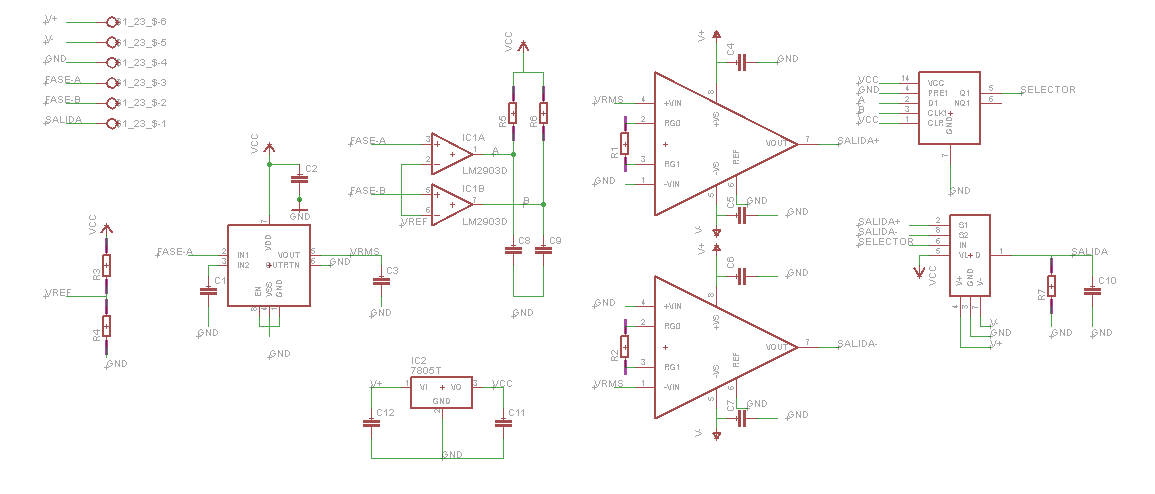
\includegraphics[scale=0.8]{FiguresP/EsquemaMotores}
\caption{Tarjeta para Mediciones de Corriente}
\label{fig:TarjetaCorriente}
\end{sidewaysfigure}



%
%Para realizar mediciones de la corriente que fluye a través de los motores se usaron sensores de corriente, los cuales producen un voltaje de salida pro proporcional a la corriente que fluye a través de ellos, con una sensibilidad de 1V/A, con lo cual en un principio se intento leer las señales de los sensores de corriente con uno de los módulos de adquisición de datos del controlador de tiempo real (ver figura \ref{fig:daq}), a través de un VI que detectara la diferencia de fase entre las dos señales de alimentación al motor(ver figura \ref{fig:señales}), y posteriormente medir el valor eficaz de una de las formas de onda. Al realizar pruebas se llego a la conclusión de que no era un método efectivo ya que era necesario emplear diez (10) entradas analógicas del modulo de adquisición de datos, es decir era necesario comprar otro modulo de entradas analógicas, y desperdiciar bastantes operaciones para encontrar un valor que fuese útil para la reflexión de fuerzas en el dispositivo maestro, con lo cual fue necesario diseñar un circuito electrónico para instrumentar dichas señales de control y pasar de tener  diez entradas analógicas a tener solo cinco, y en vez de tener formas de onda sinusoidales tener un voltaje de corriente directa proporcional (entre $\pm 4V$) a al valor eficaz de la forma de onda, con un signo positivo o negativo dependiendo del sentido de rotación del motor. 
% 









\begin{figure}
\centering
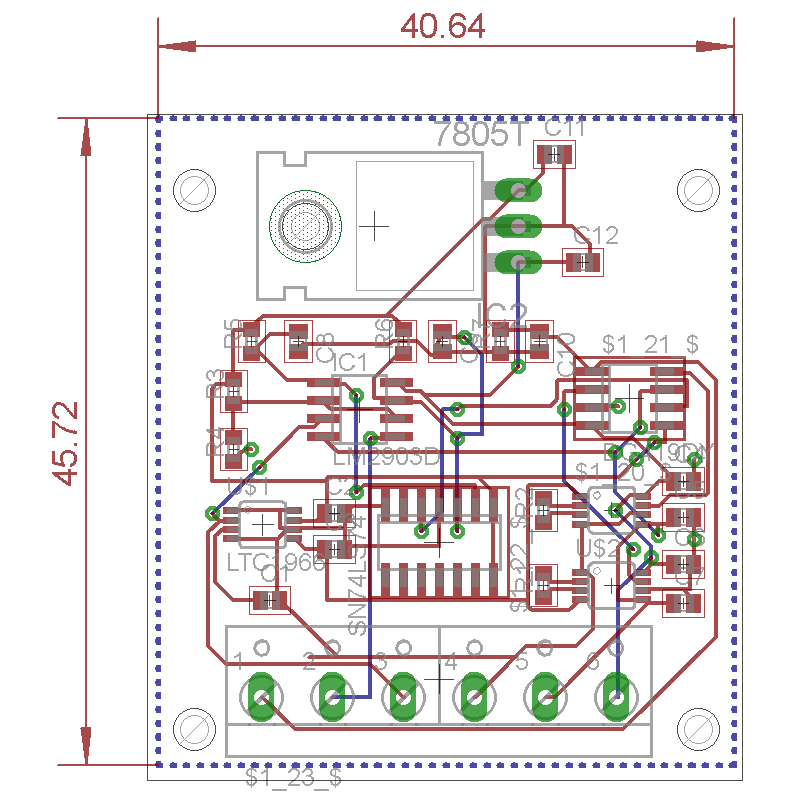
\includegraphics[scale=0.4]{FiguresP/CircuitoCorriente}
\caption{Tarjeta diseñada para el acondicionamiento de las señales de corriente en los motores}
\label{fig:TarjetaCorriente}
\end{figure}




%
%\begin{figure}
%\centering
%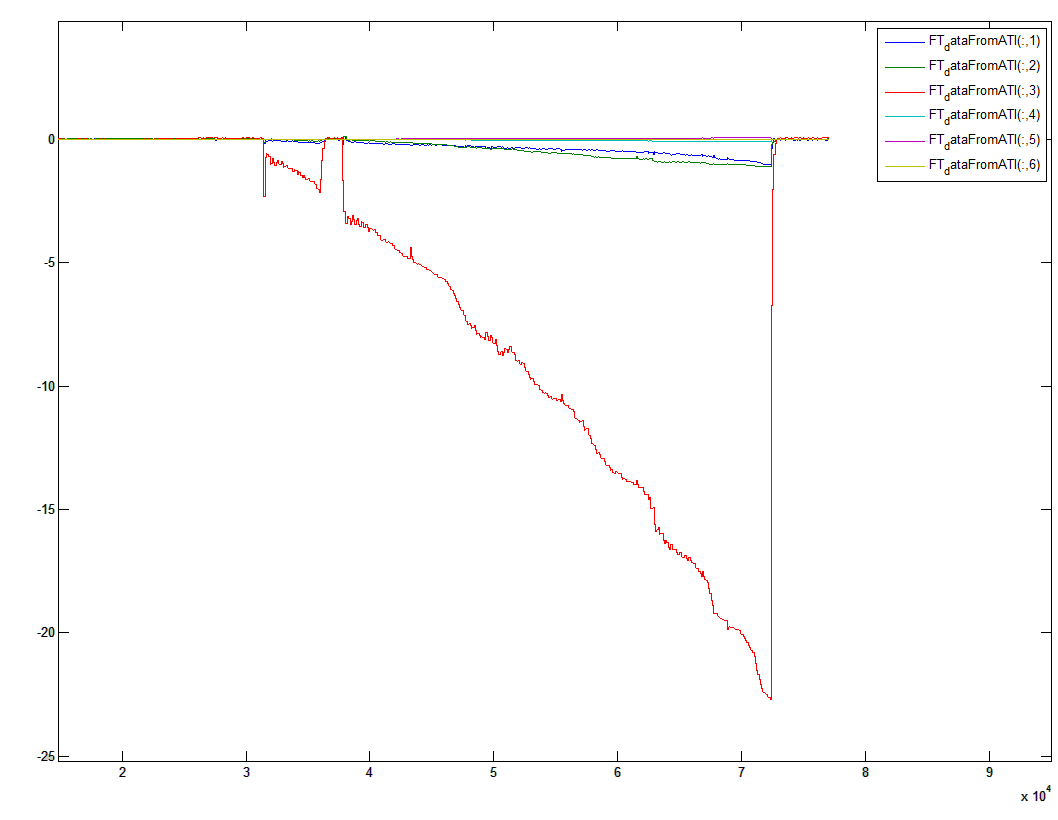
\includegraphics[scale=0.4]{FiguresP/Force}
%\caption{Tarjeta para Mediciones de Corriente}
%\label{fig:TarjetaCorriente}
%\end{figure}
%





\newpage
\section{Mediciones fuerza-corriente}
Para encontrar la relación entre la corriente que fluye por el motor y el par ejercido por el mismo se decidió montar un experimento y obtener mediciones (ver figura \ref{fig:montajeExperimento}). Para ello se utiliz\'o el sensor de fuerza ATI\textregistered SI-130 (ver figura \ref{fig:AtiForce2}), asignándose valores de corriente a través de lo motores a cada par y as\'i  encontrar una relación aproximada entre el par y la corriente consumida.


\begin{figure}[htb!]
\centering
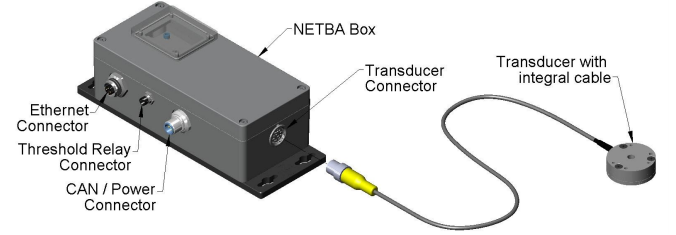
\includegraphics[scale=0.7]{Figures/AtiConnection}
\caption{Sensor de fuerza y par en seis ejes ATI\textregistered con su módulo de conexiones}
\label{fig:AtiForce2}
\end{figure}

El sensor ATI \textregistered permite mediciones de par y fuerza en seis ejes gracias a su celda de carga multi-eje. El sensor cuenta con un sistema de adquisición de datos inteligente al que se puede acceder a través de una interfaz Ethernet/DeviceNet. Los rangos de medición así como las resoluciones máximas en cada uno de los ejes del sensor se muestran en la tabla \ref{tab:ati}\\

\begin{table}[htb!]
\begin{flushleft}
\begin{tabular}{ c c c c c c c c  }
& & Rango de Sensibilidad   &  &  &  &   Resolución  &\\
\hline
Calibración &	Fx,Fy &	Fz     &	Tx,Ty &	Tz	  & Fx,Fy  &	Fz	    &  Tx,Ty,Tz \\
\hline
SI-130-10	& 130 N   &	400 N  & 10 Nm  &	10 Nm  &	1/40 N &	1/20 N 	& 1/800 Nm  \\
\hline
\end{tabular}
\end{flushleft}
\caption{Calibración métrica  (SI)  del Sensor ATI}
\label{tab:ati}
\end{table}


Para realizar la adquisición de datos fue necesario crear una interfaz visual (del ingl\'es \textit{ Interfase} VI) en Labview para capturar de manera paralela las lecturas de los sensores de corriente y la información acerca de la fuerza en un eje del sensor ATI. El VI diseñado est\'a encargado de establecer una conexión ethernet entre ambos dispositivos y capturando los datos en un archivo \textbf{.mat} de Matlab, para posteriormente hacer el tratamiento de los mismo y hacer un ajuste de curva.\\


\begin{figure}[htb!]
%\subfigure[Montaje para la medición de fuerza del sensor $ATI^{\textregistered}$]{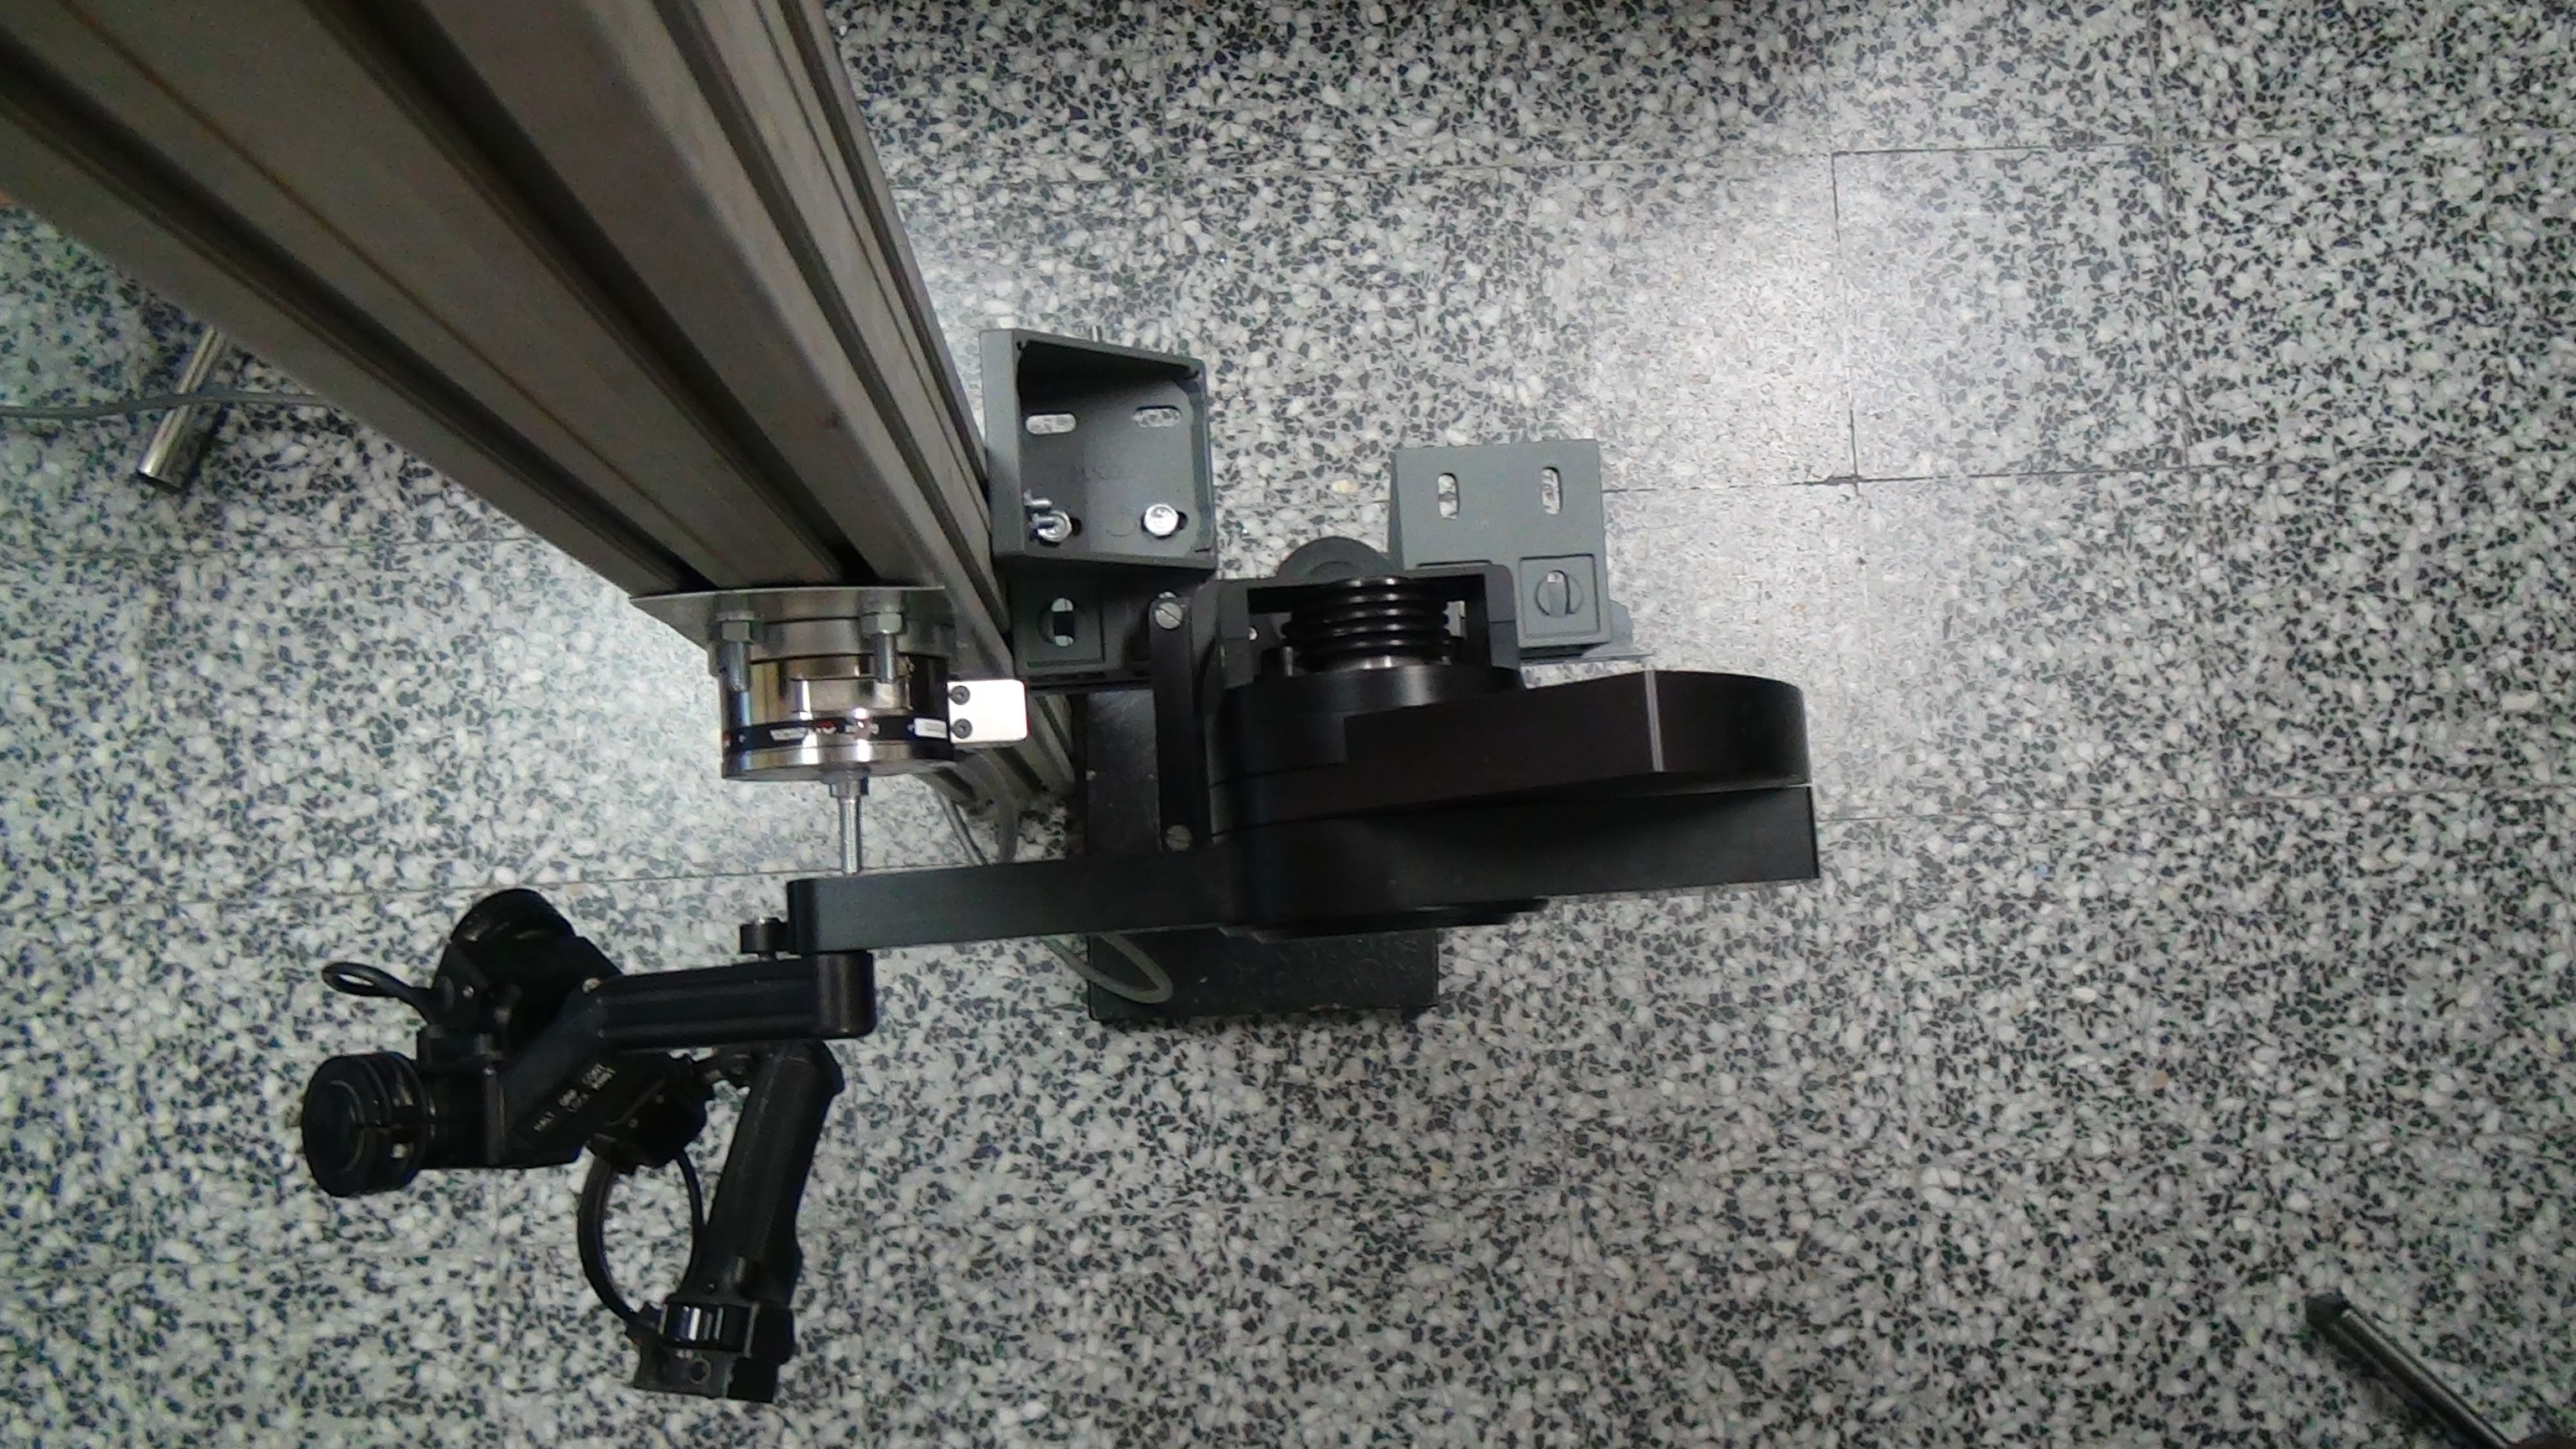
\includegraphics[scale=0.12]{FiguresP/setupTorque1}\label{fig:current}}

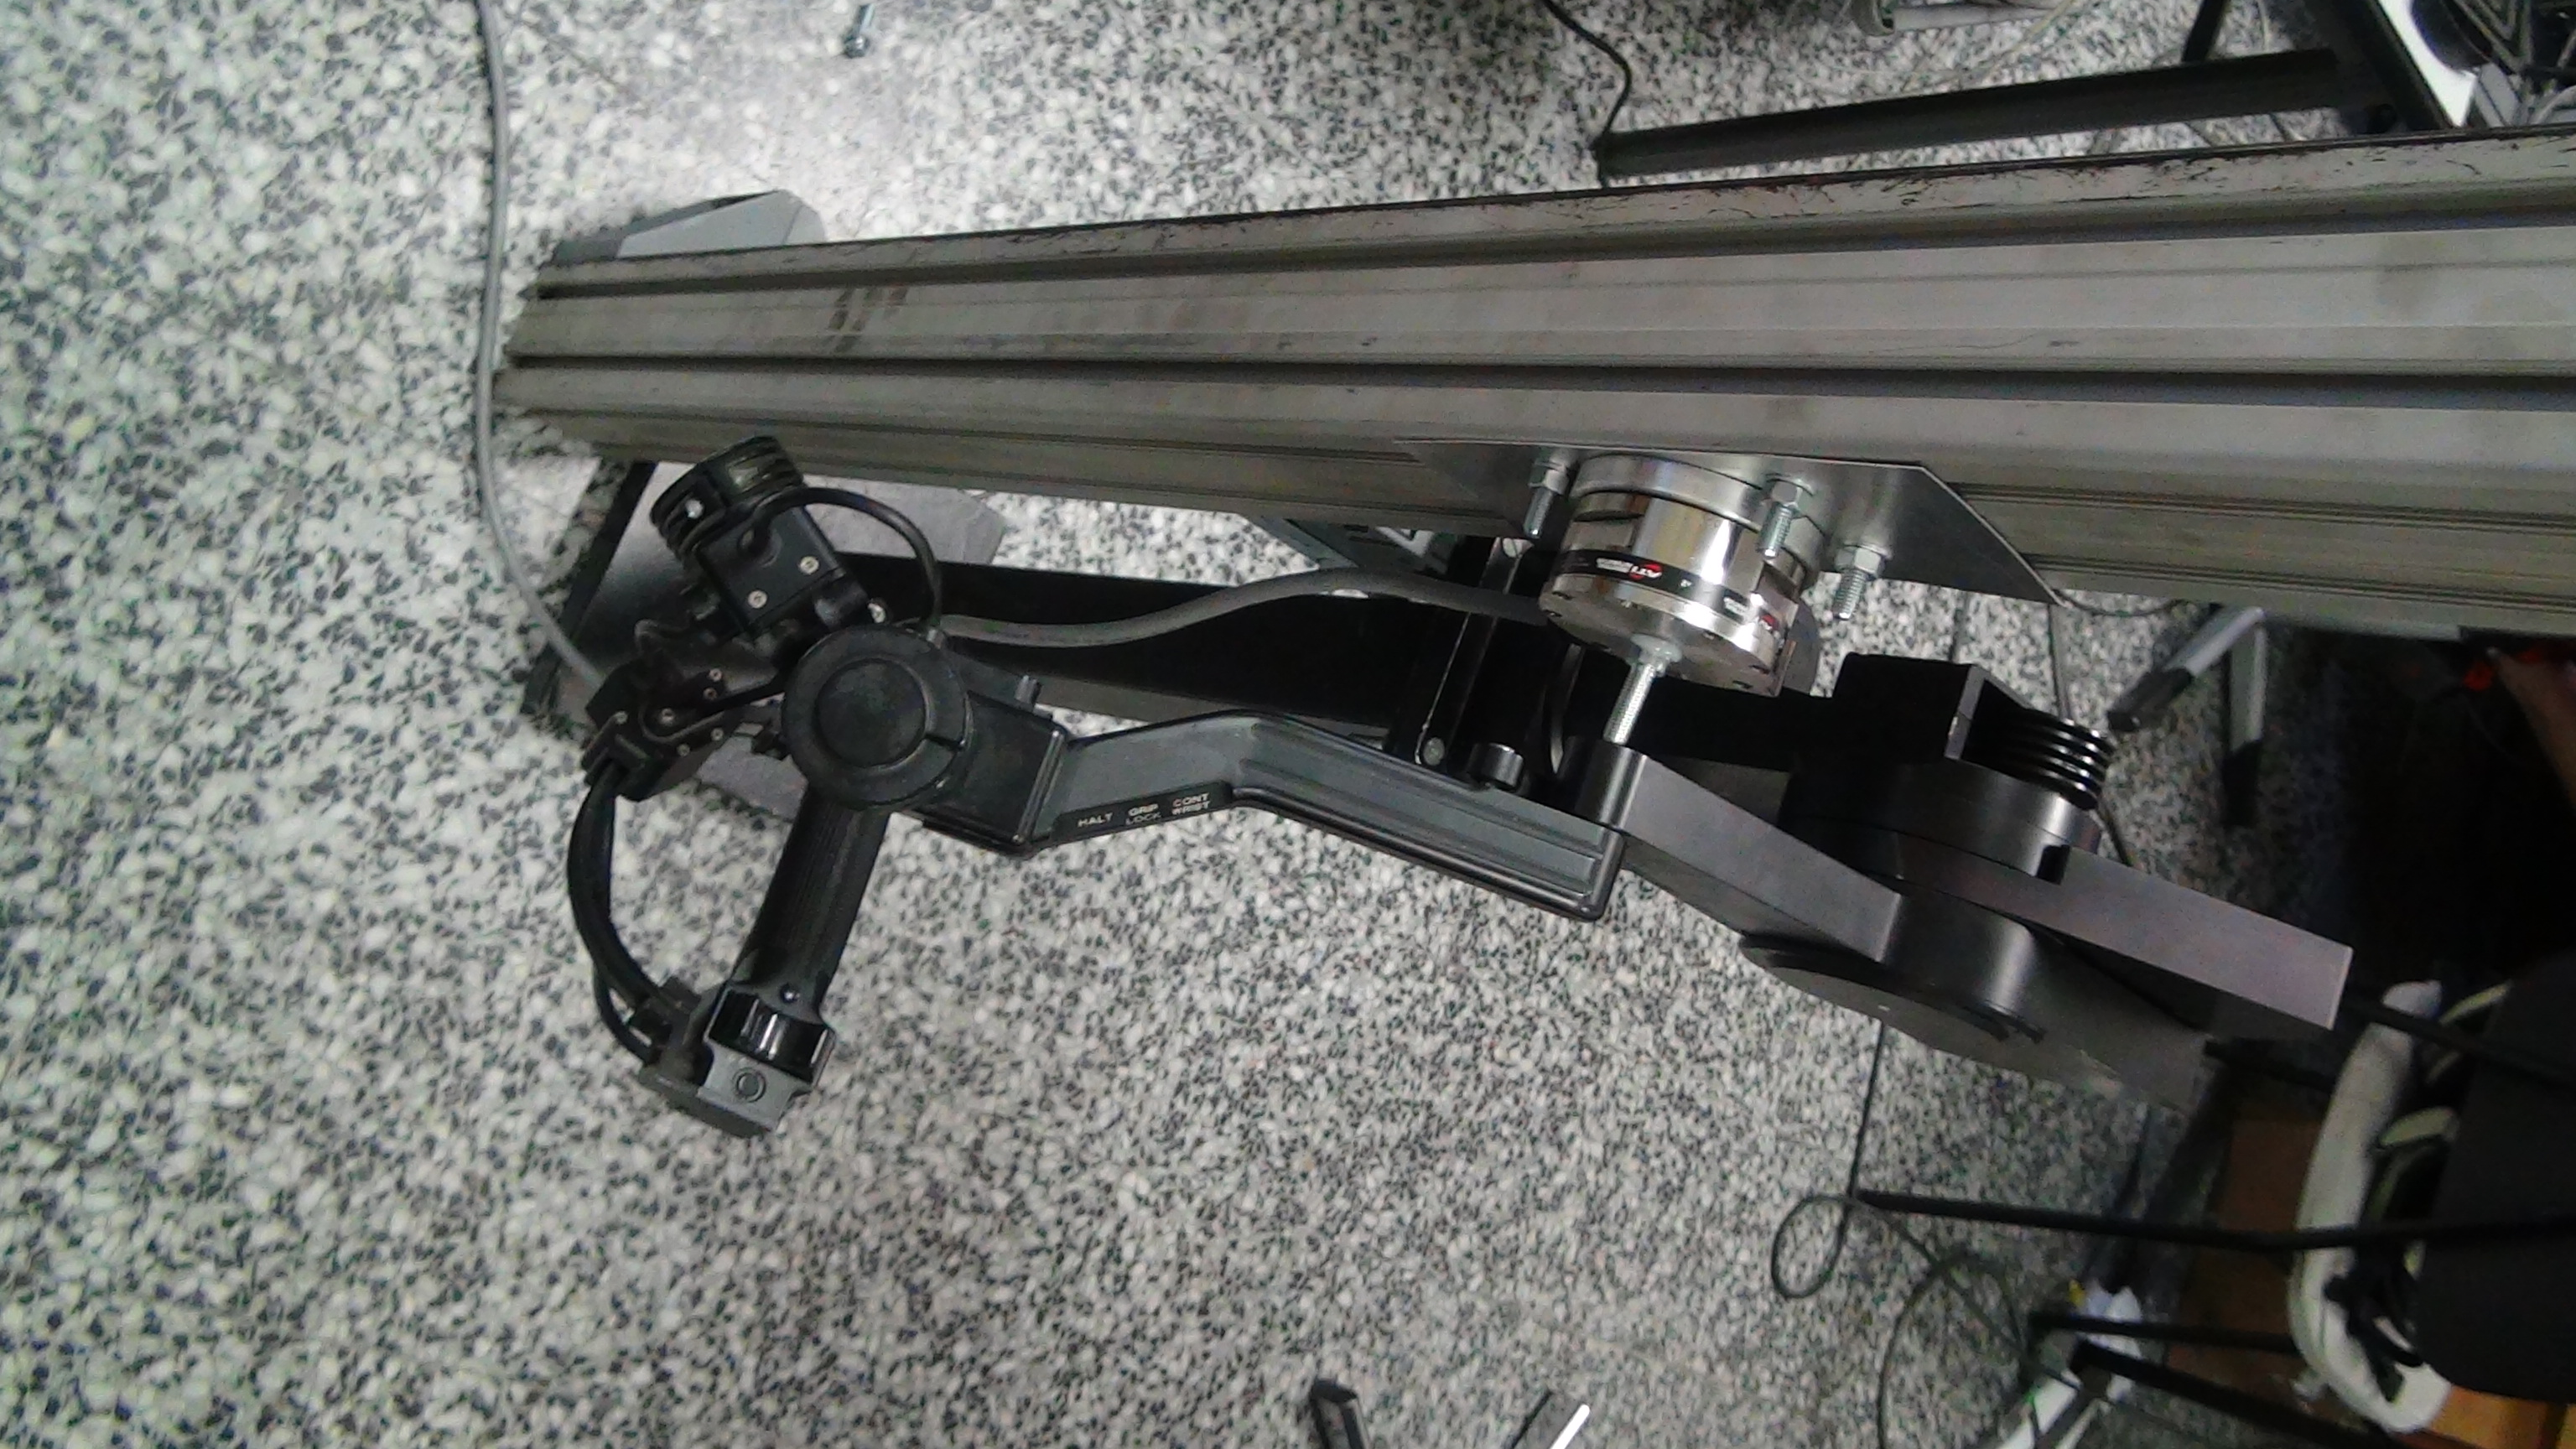
\includegraphics[scale=0.12]{FiguresP/setupTorque2}\label{fig:force}
\caption{Montaje del experimento para la medición de fuerza de la fuerza ejercida por el maestro usando el sensor $ATI^{\textregistered}$}
\label{fig:montajeExperimento}
\end{figure}

%\section{Mediciones de Par ejercido por los Motores con el sensor ATI\textregistered}

%\begin{figure}[htb!]
%\centering
%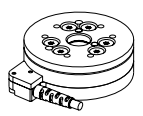
\includegraphics[scale=0.5]{Figures/AtiSensor}
%\caption{Sensor de Fuerza y Torque en seis ejes ATI\textregistered}
%\label{fig:AtiForce}
%\end{figure}


%\newpage
%\begin{figure}
%\subfigure[Corriente Medida a traves las tarjetas diseñadas]{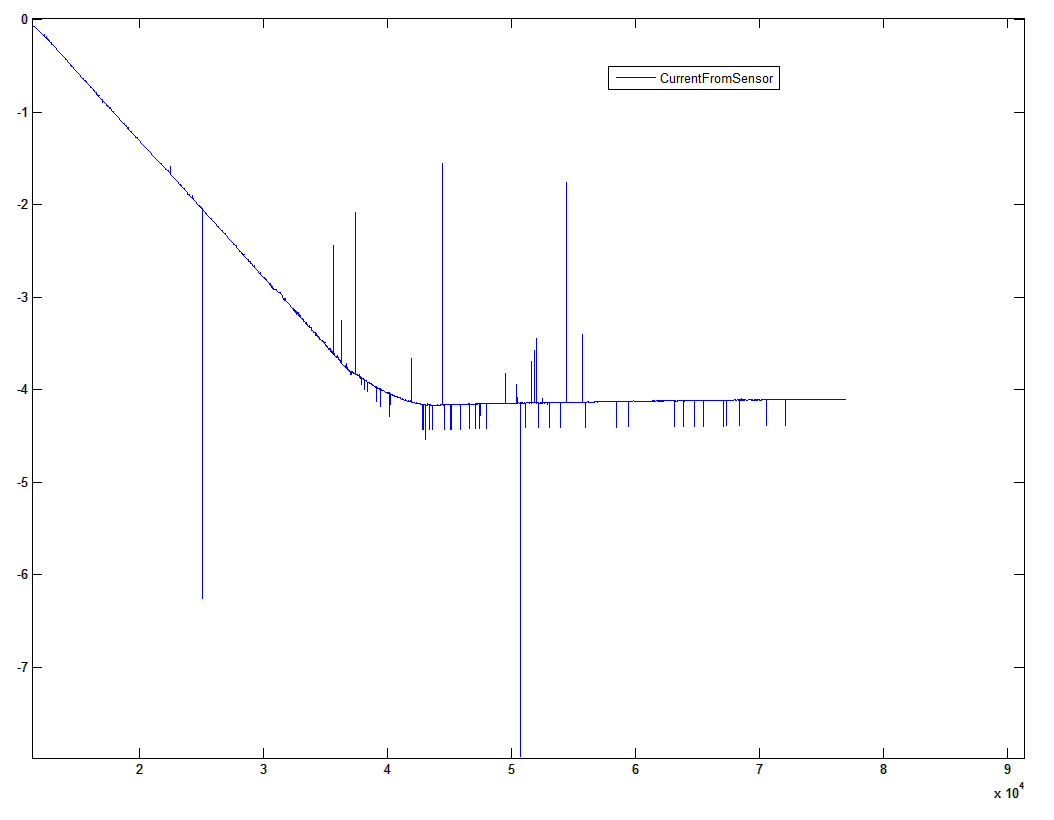
\includegraphics[scale=0.4]{FiguresP/Current}\label{fig:current}}
%\subfigure[Medicion de fuerza del sensor $ATI^{\textregistered}$]{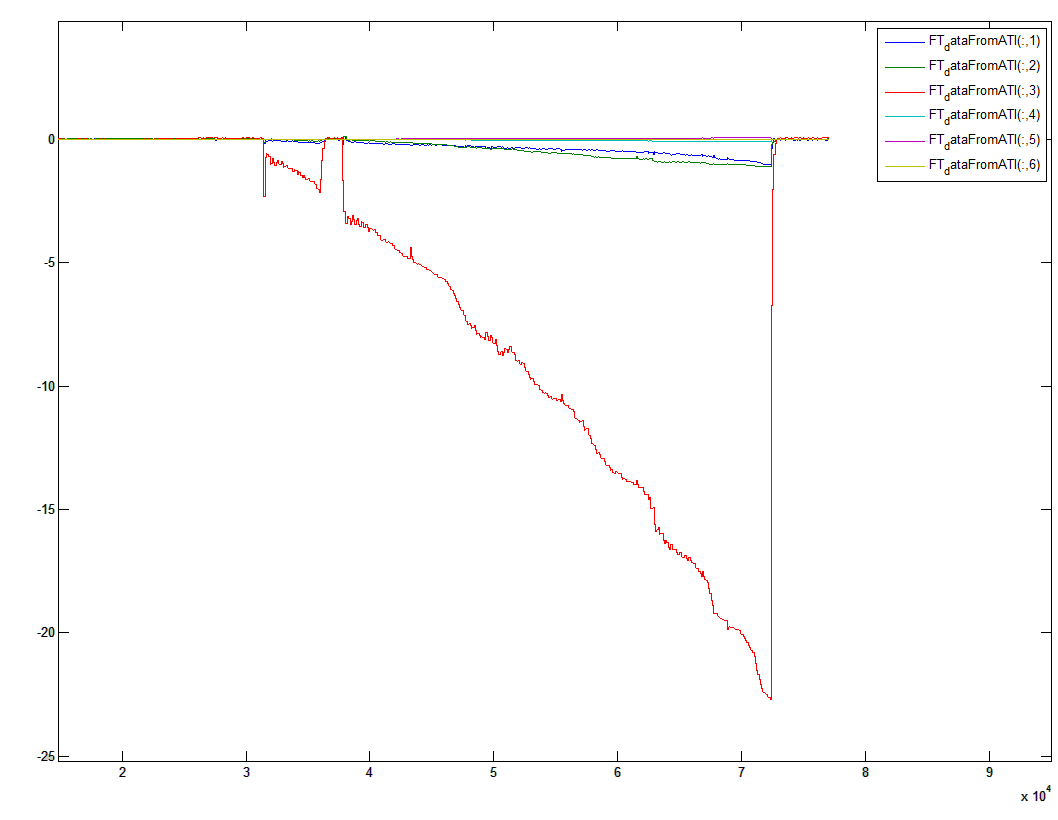
\includegraphics[scale=0.4]{FiguresP/Force}\label{fig:force}}
%\caption{Mediciones obtenidas del experimento para determinar la relacion entre la corriente y el par}
%\end{figure}


\newpage
\section{Modelo del motor Corriente VS Fuerza}
Con los datos obtenidos a partir de las mediciones del experimento se obtuvo un ajuste de curva usando Matlab. Los datos obtenidos de los sensores pueden verse en la figura \ref{fig:MedicionesFuerzaCorriente}. El eje de las \textbf{X} es el tiempo transcurrido durante el experimento mientras que el eje de las \textbf{Y} corresponde a los valores obtenidos de ambos sensores. Para el caso del sensor de fuerza la magnitud se dividió entre diez para una mayor comodidad a la hora de ver la gráfica.




\begin{figure}[htb!]
\centering
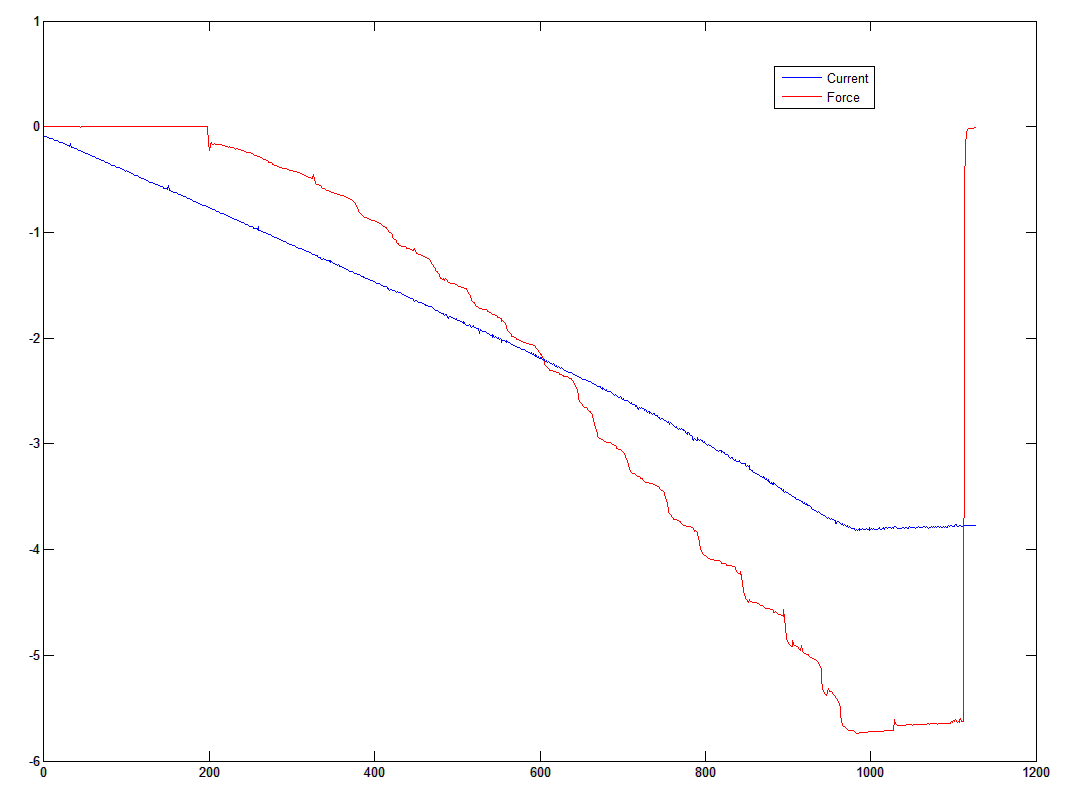
\includegraphics[scale=0.4]{FiguresP/ForceCurrent}
\caption{Tarjeta para mediciones de corriente}
\label{fig:MedicionesFuerzaCorriente}
\end{figure}


A partir de una aproximación por mínimos cuadrados se encontró la ecuación que relaciona la fuerza de los motores con la corriente:

\subsection*{Modelo lineal}

\begin{equation}
f(x) = p_1x + p_2
\end{equation}
     
coeficientes (con unos límites de confianza del 95\% ):
		$$       p_1 =       17.93  (17.51, 18.34)$$       
       $$       p_2 =      -15.65  (-16.73, -14.58) $$
  Calidad de la aproximación:\\
  SSE: 4.646e+004\\
  R-cuadrada: 0.8794\\
  R-cuadrada ajustada: 0.8792\\  
  RMSE: 6.903


\subsection*{Modelo cuadrático}
\begin{equation}
     f(x) = p_1 x^2 + p_2x + p_3
\end{equation}

Coeficientes (con unos límites de confianza del 95\% ):
$$     p_1 =      0.8509  (0.3606, 1.341)$$
$$       p_2 =       13.92  (11.57, 16.26)$$       
$$       p_3 =      -11.85  (-14.29, -9.41)$$

  Calidad de la aproximación:\\
  SSE: 4.592e+004\\
  R-cuadrada: 0.8808\\
  R-cuadrada ajustada: 0.8805\\
  RMSE: 6.866





\begin{figure}[htb!]
\centering
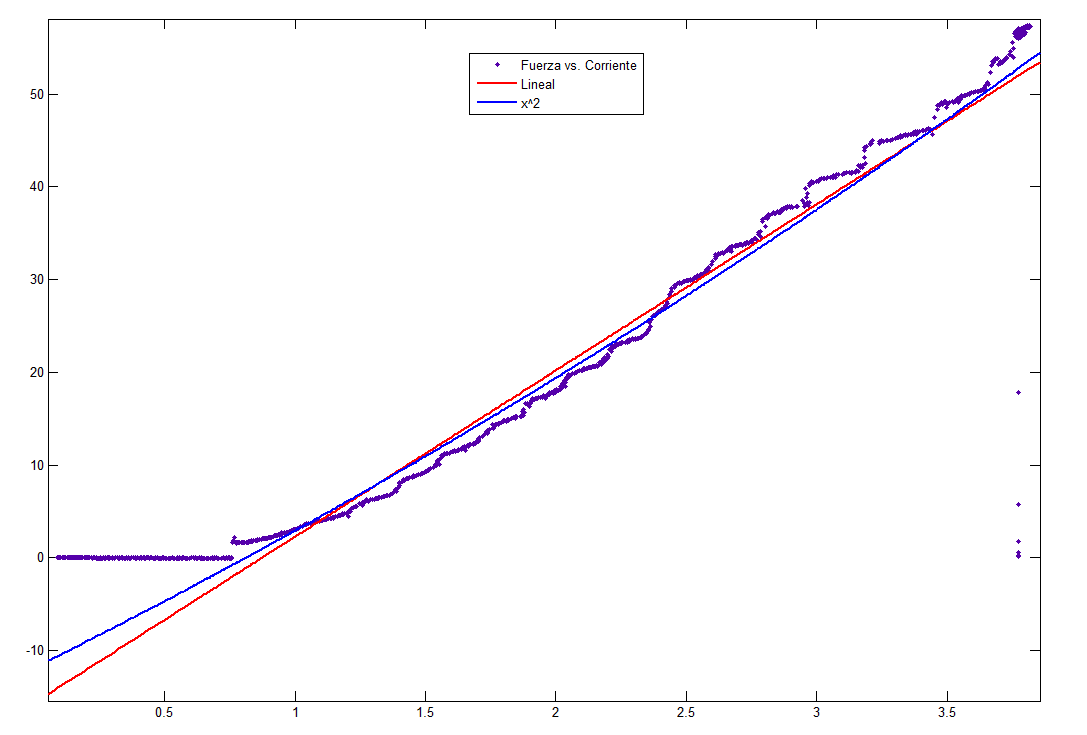
\includegraphics[scale=0.5]{FiguresP/ModeloFC}
\caption{Modelos hecho por aproximación de mínimos cuadrados}
\label{fig:curveFitting}
\end{figure}

Analizando la figura \ref{fig:curveFitting} se concluye que no existe mucha diferencia entre el modelo lineal y el modelo cuadrático, con lo cual es preferible usar el modelo lineal para simplificar las operaciones.

%\section{Caracterización del sistema Maestro}
%Posterior al diseño del circuito electrónico para la medición de corriente en los motores de cada una de las articulaciones del sistema maestro.


\section{Bucle de Control en Fuerza}

Para la reflexión de fuerzas en el maestro del manipulador grips se propone el uso de un regulador proporcional integral con las siguientes ganancias:

\begin{equation}
K=3.00 \qquad    T_i=0.001s \qquad   dt=0.001s
\end{equation}



\begin{figure}[htb!]
\centering
\caption{Esquema de control en corriente de los motores del dispositivo maestro}
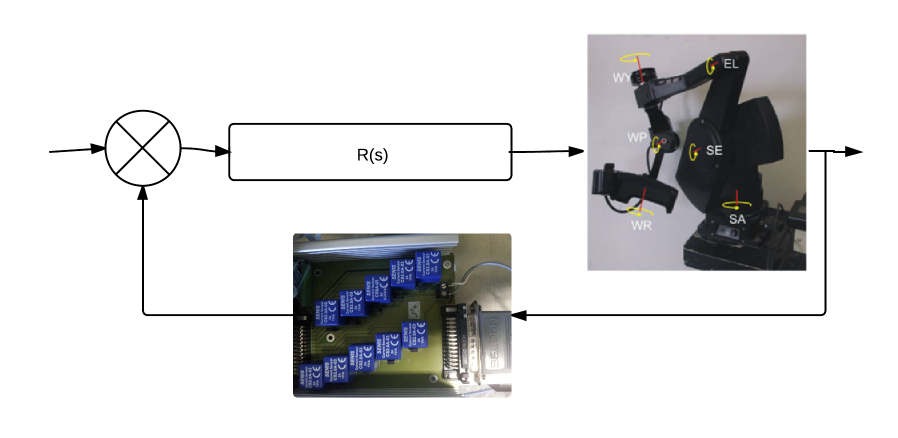
\includegraphics[scale=0.5]{FiguresP/Controller}
\end{figure}




